\section{联合收敛}
\label{sec:weak-joint}

设$X_n\xrightarrow{\mathrm{d}}X$，$Y_n\xrightarrow{\mathrm{d}}Y$。$X_n+Y_n$的极限是什么？这个问题在只知道两个边缘极限时没有答案，因为$X+Y$的分布取决于$X$与$Y$怎样配对，而边缘分布不含配对的信息。本节先把联合收敛与边缘收敛分开，再给出两类常用的判据：方向投影，以及一个分量趋于常量的情形。有了联合极限，上一节的连续映射定理就可以处理和、积与比。

\subsection{边缘收敛与联合收敛}
\label{sec:weak-marginal-joint}

设$(\bm{X}_n,\bm{Y}_n)$是取值于$\mathbb{R}^{d}\times\mathbb{R}^{k}$的随机向量，即每个$n$下$\bm{X}_n$与$\bm{Y}_n$定义在同一个概率空间上。联合收敛$(\bm{X}_n,\bm{Y}_n)\xrightarrow{\mathrm{d}}(\bm{X},\bm{Y})$就是这个$(d+k)$维随机向量的依分布收敛。坐标投影$(\bm{x},\bm{y})\mapsto\bm{x}$连续，由连续映射定理，联合收敛推出$\bm{X}_n\xrightarrow{\mathrm{d}}\bm{X}$与$\bm{Y}_n\xrightarrow{\mathrm{d}}\bm{Y}$。

反过来不成立。设$Z\sim\mathcal{N}(0,1)$，令
\[
 X_n=Z,\qquad Y_n=(-1)^{n}Z .
\]
$-Z$也服从$\mathcal{N}(0,1)$，所以两个边缘分布对每个$n$都是$\mathcal{N}(0,1)$，边缘平凡地收敛。联合分布却在两种之间交替：偶数$n$时$(Z,Z)$落在直线$y=x$上，奇数$n$时$(Z,-Z)$落在$y=-x$上。取有界连续函数$f(x,y)=\min(1,\lvert x-y\rvert)$，偶数项的读数为$0$，奇数项为$\mathbb{E}[\min(1,2\lvert Z\rvert)]>0$，所以联合分布没有极限。图~\ref{fig:weak-pairings}画出这两种配对，以及同样边缘下的第三种配对：独立。

\begin{BookInlineFigure}
 \centering
 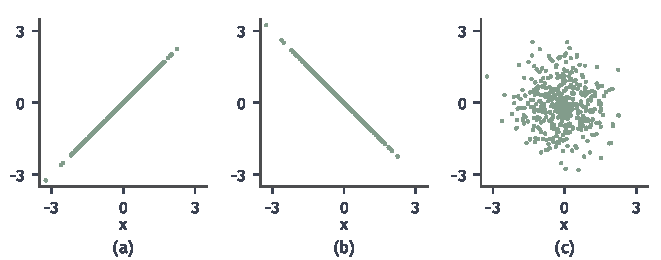
\includegraphics[width=112mm]{figures/07-probability/03-probability-limits/matplotlib/weak-pairings/figure.pdf}
 \caption{边缘相同、配对不同。三幅图各有$400$个样本点（种子$7$），两个坐标的边缘分布都是$\mathcal{N}(0,1)$。(a)$(Z,Z)$；(b)$(Z,-Z)$；(c)$(Z,Z')$，$Z'$与$Z$独立同分布。}
 \label{fig:weak-pairings}
\end{BookInlineFigure}

\paragraph{各分量独立的情形}
若对每个$n$，$\bm{X}_n$与$\bm{Y}_n$独立，配对方式就被固定下来，边缘收敛足以推出联合收敛。

\begin{theorem}[独立分量的联合极限]
\label{thm:weak-independent-joint}
设对每个$n$，$\bm{X}_n$与$\bm{Y}_n$定义在同一概率空间上且相互独立，$\bm{X}_n\xrightarrow{\mathrm{d}}\bm{X}$，$\bm{Y}_n\xrightarrow{\mathrm{d}}\bm{Y}$。则$(\bm{X}_n,\bm{Y}_n)\xrightarrow{\mathrm{d}}(\bm{X},\bm{Y})$，其中$\bm{X}$与$\bm{Y}$独立，即极限分布是$P_{\bm{X}}$与$P_{\bm{Y}}$的乘积。
\end{theorem}

\begin{proof}
由式~\eqref{eq:weak-cf-joint-independent}与连续性定理的(1)，
\[
 \phi_{(\bm{X}_n,\bm{Y}_n)}(\bm{s},\bm{t})=\phi_{\bm{X}_n}(\bm{s})\,\phi_{\bm{Y}_n}(\bm{t})\longrightarrow\phi_{\bm{X}}(\bm{s})\,\phi_{\bm{Y}}(\bm{t}) .
\]
取$\bm{X}$与$\bm{Y}$独立，右边正是$(\bm{X},\bm{Y})$的特征函数，它连续。由连续性定理的(2)，结论成立。
\end{proof}

定理只要求同一个$n$下的两个分量独立，不要求不同$n$之间有任何关系；各个$n$甚至可以在不同的概率空间上。例如每个$n$下独立地取$X_n\sim\operatorname{Bin}(n,2/n)$与格点均匀分布$U_n$，则$(X_n,U_n)$依分布收敛到$\operatorname{Poisson}(2)$与$\operatorname{Unif}(0,1)$的乘积分布。

\subsection{Cramér--Wold判据}
\label{sec:weak-cramer-wold}

一般的联合分布怎样检验？直接用多元特征函数可以，但常常更方便的是把向量投影到一个方向上，化为一维问题。投影$\langle\bm{a},\bm{X}\rangle$的特征函数在$1$处的值是
\[
 \phi_{\langle\bm{a},\bm{X}\rangle}(1)=\mathbb{E}\bigl[\mathrm{e}^{\mathrm{i}\langle\bm{a},\bm{X}\rangle}\bigr]=\phi_{\bm{X}}(\bm{a}) .
\]
所以多元特征函数在$\bm{a}$处的值，就是沿方向$\bm{a}$的一维投影的信息。知道所有方向的投影分布，就知道整个多元特征函数。

\begin{theorem}[Cramér--Wold判据]
\label{thm:weak-cramer-wold}
设$\bm{X}_n,\bm{X}$取值于$\mathbb{R}^{d}$。则$\bm{X}_n\xrightarrow{\mathrm{d}}\bm{X}$，当且仅当对每个$\bm{a}\in\mathbb{R}^{d}$，
\begin{equation}
 \langle\bm{a},\bm{X}_n\rangle\xrightarrow{\mathrm{d}}\langle\bm{a},\bm{X}\rangle .
 \label{eq:weak-cramer-wold}
\end{equation}
特别地，$\bm{X}$的分布由全部一维投影$\langle\bm{a},\bm{X}\rangle$的分布确定。
\end{theorem}

\begin{proof}
必要性：$\bm{x}\mapsto\langle\bm{a},\bm{x}\rangle$连续，由连续映射定理。充分性：由式~\eqref{eq:weak-cramer-wold}与连续性定理的(1)，对每个$\bm{a}$，
\[
 \phi_{\bm{X}_n}(\bm{a})=\phi_{\langle\bm{a},\bm{X}_n\rangle}(1)\longrightarrow\phi_{\langle\bm{a},\bm{X}\rangle}(1)=\phi_{\bm{X}}(\bm{a}) .
\]
极限$\phi_{\bm{X}}$连续，由连续性定理的(2)得$\bm{X}_n\xrightarrow{\mathrm{d}}\bm{X}$。最后一句：若$\bm{X}$与$\bm{Y}$的各个投影同分布，则$\phi_{\bm{X}}(\bm{a})=\phi_{\bm{Y}}(\bm{a})$对一切$\bm{a}$成立，由定理~\ref{thm:weak-cf-uniqueness}得$P_{\bm{X}}=P_{\bm{Y}}$。
\end{proof}

这个判据也称为\term{Cramér--Wold方法}（Cramér--Wold device）。判据要求所有方向，坐标方向只是$\bm{a}=\bm{e}_j$这$d$个特例，它们只给出边缘分布。上一小节的例子已经说明边缘不够；下面看一个固定的随机向量，它的坐标方向都是高斯，某个斜方向却不是。

\paragraph{联合高斯的判别}
第~\ref{chap:multivariate-distributions}章说过：若每个线性组合$\langle\bm{a},\bm{X}\rangle$都服从一元高斯分布（方差可以为$0$），则$\bm{X}$联合高斯。现在可以证明。每个坐标服从高斯分布，所以二阶矩有限，记$\bm{\mu}=\mathbb{E}[\bm{X}]$，$\bm{\Sigma}$为协方差矩阵。$\langle\bm{a},\bm{X}\rangle$的均值为$\langle\bm{a},\bm{\mu}\rangle$，方差为$\bm{a}^{\top}\bm{\Sigma}\bm{a}$，按假设它是高斯的，于是
\[
 \phi_{\bm{X}}(\bm{a})=\phi_{\langle\bm{a},\bm{X}\rangle}(1)=\exp\Bigl(\mathrm{i}\langle\bm{a},\bm{\mu}\rangle-\frac12\bm{a}^{\top}\bm{\Sigma}\bm{a}\Bigr) .
\]
这正是式~\eqref{eq:weak-mvn-cf}中$\mathcal{N}(\bm{\mu},\bm{\Sigma})$的特征函数，由定理~\ref{thm:weak-cf-uniqueness}，$\bm{X}\sim\mathcal{N}(\bm{\mu},\bm{\Sigma})$。

那一章还给出了只检查坐标方向不够的例子。$Z\sim\mathcal{N}(0,1)$，$S$以各$1/2$的概率取$\pm1$且与$Z$独立，$\bm{X}=(Z,SZ)$。两个坐标都服从$\mathcal{N}(0,1)$，由独立性，协方差$\mathbb{E}[SZ^{2}]$等于$\mathbb{E}[S]\,\mathbb{E}[Z^{2}]=0$。若$\bm{X}$联合高斯，它就是$\mathcal{N}(\bm{0},\bm{I}_2)$，方向$\bm{a}=(1,1)$上的投影应服从$\mathcal{N}(0,2)$。实际上
\[
 Z+SZ=(1+S)Z=\begin{cases}2Z,&S=1,\\0,&S=-1,\end{cases}
\]
它以概率$1/2$恰好等于$0$，不是高斯分布。图~\ref{fig:weak-cramer-wold}(a)是$\bm{X}$的样本，全部落在两条对角线上；(b)是这个斜方向投影的分布。

\begin{BookInlineFigure}
 \centering
 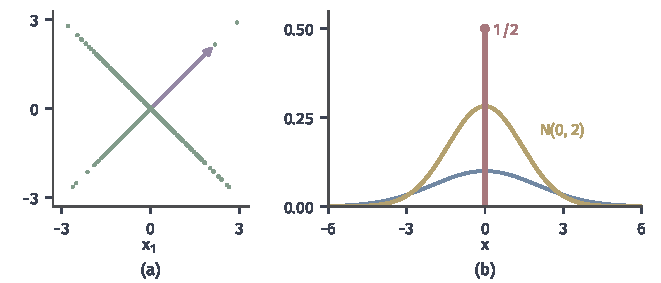
\includegraphics[width=112mm]{figures/07-probability/03-probability-limits/matplotlib/weak-cramer-wold/figure.pdf}
 \caption{坐标方向都是高斯，斜方向不是。(a)$\bm{X}=(Z,SZ)$的$600$个样本（种子$11$），两个边缘都是$\mathcal{N}(0,1)$，紫色箭头为方向$(1,1)$。(b)$Z+SZ$的分布：$0$处质量$1/2$的原子（红色竖线），其余质量的密度为$\frac12$乘$\mathcal{N}(0,4)$的密度（蓝）；黄线为假如联合高斯时应有的$\mathcal{N}(0,2)$密度。}
 \label{fig:weak-cramer-wold}
\end{BookInlineFigure}

Cramér--Wold判据适用于固定的有限维数$d$。下一章的多元中心极限定理正是用它把各个方向上的一维极限合成联合高斯极限。

\subsection{Slutsky定理}
\label{sec:weak-slutsky}

联合收敛有一个特别好用的情形：一个分量依分布收敛，另一个依概率趋于常量。常量没有随机性，不存在配对问题，所以边缘信息就够了。典型的场合是用一个依概率收敛的量替换未知的常数，例如第~\ref{chap:laws-of-large-numbers}章的大数律给出的样本平均。

\begin{theorem}[Slutsky定理]
\label{thm:weak-slutsky}
设对每个$n$，$\bm{X}_n$与$\bm{Y}_n$定义在同一概率空间上，分别取值于$\mathbb{R}^{d}$与$\mathbb{R}^{k}$。若$\bm{X}_n\xrightarrow{\mathrm{d}}\bm{X}$，且对常向量$\bm{c}\in\mathbb{R}^{k}$有$\bm{Y}_n\xrightarrow{\mathbb{P}}\bm{c}$，则
\begin{equation}
 (\bm{X}_n,\bm{Y}_n)\xrightarrow{\mathrm{d}}(\bm{X},\bm{c}) .
 \label{eq:weak-slutsky-joint}
\end{equation}
因此，对实随机变量$X_n\xrightarrow{\mathrm{d}}X$与$Y_n\xrightarrow{\mathbb{P}}c$，
\begin{equation}
 X_n+Y_n\xrightarrow{\mathrm{d}}X+c,\qquad Y_nX_n\xrightarrow{\mathrm{d}}cX,\qquad X_n/Y_n\xrightarrow{\mathrm{d}}X/c\quad(c\neq0) .
 \label{eq:weak-slutsky}
\end{equation}
\end{theorem}

\begin{proof}
由Portmanteau定理的(2)，只需对有界Lipschitz函数$f$验证。设$\lvert f\rvert\leq M$，Lipschitz常数为$L$。任取$\varepsilon>0$，把差拆成两部分：
\[
 \begin{aligned}
 \bigl\lvert\mathbb{E}[f(\bm{X}_n,\bm{Y}_n)]-\mathbb{E}[f(\bm{X},\bm{c})]\bigr\rvert
 &\leq\mathbb{E}\bigl[\lvert f(\bm{X}_n,\bm{Y}_n)-f(\bm{X}_n,\bm{c})\rvert\bigr]\\
 &\quad+\bigl\lvert\mathbb{E}[f(\bm{X}_n,\bm{c})]-\mathbb{E}[f(\bm{X},\bm{c})]\bigr\rvert .
 \end{aligned}
\]

第一部分在$\lVert\bm{Y}_n-\bm{c}\rVert_2<\varepsilon$时被$L\varepsilon$控制，其余情形被$2M$控制，所以不超过
\[
 L\varepsilon+2M\,\mathbb{P}\bigl(\lVert\bm{Y}_n-\bm{c}\rVert_2\geq\varepsilon\bigr) ,
\]
后一项趋于零。第二部分中，$\bm{x}\mapsto f(\bm{x},\bm{c})$有界连续，由$\bm{X}_n\xrightarrow{\mathrm{d}}\bm{X}$趋于零。于是左边的上极限不超过$L\varepsilon$，$\varepsilon$任意，式~\eqref{eq:weak-slutsky-joint}成立。

式~\eqref{eq:weak-slutsky}中，$(x,y)\mapsto x+y$与$(x,y)\mapsto xy$连续。$(x,y)\mapsto x/y$只在直线$y=0$上不连续，而$(X,c)$落在这条直线上的概率在$c\neq0$时为零。由连续映射定理即得。
\end{proof}

\term{Slutsky定理}（Slutsky's theorem）不要求$\bm{X}_n$与$\bm{Y}_n$独立，它们可以有任意的依赖关系；证明的第一部分只用了$\bm{Y}_n$靠近$\bm{c}$的概率，没有用到$\bm{Y}_n$与$\bm{X}_n$怎样配对。这里只需要每个$n$下二者在同一空间上，使$(\bm{X}_n,\bm{Y}_n)$有意义。

看一个强依赖的例子。设$X\sim\mathcal{N}(0,1)$，令$X_n=X$，$Y_n=1+X/\sqrt{n}$。则$Y_n-1=X/\sqrt n\to0$对每个样本点成立，$Y_n\xrightarrow{\mathbb{P}}1$，而$Y_n$完全由$X_n$决定。$\mathbb{P}(Y_n=0)=0$，比值有定义，由Slutsky定理，
\[
 \frac{X_n}{Y_n}=\frac{X}{1+X/\sqrt{n}}\xrightarrow{\mathrm{d}}\mathcal{N}(0,1) .
\]
有限的$n$下，分母可能很接近$0$，比值有很重的尾部；$n$增大，这种情形的概率越来越小。图~\ref{fig:weak-slutsky}用模拟显示了这个过程。

\begin{BookInlineFigure}
 \centering
 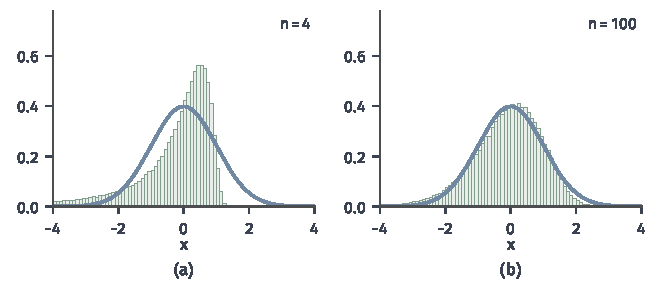
\includegraphics[width=112mm]{figures/07-probability/03-probability-limits/matplotlib/weak-slutsky/figure.pdf}
 \caption{Slutsky定理中的依赖分母。$X\sim\mathcal{N}(0,1)$，$X/(1+X/\sqrt n)$的直方图（浅绿，$2\times10^{5}$个样本，种子$3$，只画$[-4,4]$内的部分），蓝线为$\mathcal{N}(0,1)$的密度。(a)$n=4$，左侧的长尾来自分母接近零的样本；(b)$n=100$。}
 \label{fig:weak-slutsky}
\end{BookInlineFigure}

\paragraph{条件的作用}
常量分母必须非零。$X_n=Z\sim\mathcal{N}(0,1)$，$Y_n=1/n\xrightarrow{\mathbb{P}}0$，则$X_n/Y_n=nZ\sim\mathcal{N}(0,n^{2})$，质量逃向无穷远，没有弱极限。

常量也不能换成一般的随机极限。设$X_n=Z$，$Y_n=(-1)^{n}Z$，则$X_n\xrightarrow{\mathrm{d}}Z$，$Y_n\xrightarrow{\mathrm{d}}Z$，但
\[
 X_n+Y_n=\begin{cases}2Z,&n\text{为偶数},\\0,&n\text{为奇数}\end{cases}
\]
没有极限。两个分量各自依分布收敛到非退化的分布时，必须另外知道它们的联合收敛，例如由定理~\ref{thm:weak-independent-joint}的独立条件或由Cramér--Wold判据得到，才能谈论和的极限。
